\documentclass[10pt,fleqn]{scrartcl}

\usepackage{fullpage}
\usepackage{amsmath}
\usepackage{amsthm}
\usepackage{helvet}
\usepackage{hyperref}

\usepackage{upquote}

\newtheoremstyle{exstyle}% style name
{2ex}% above space
{2ex}% below space
{}% body font
{}% indent amount
{\bfseries}% head font
{}% post head punctuation
{\newline}% post head punctuation
{}% head spec
\theoremstyle{exstyle}
\newtheorem{exercise}{Exercise}

\usepackage{tcolorbox}
\tcbuselibrary{theorems,skins,breakable}

\tcolorboxenvironment{exercise}{
enhanced jigsaw,colframe=black,interior hidden,
breakable,before skip=10pt,after skip=10pt }

\usepackage{datetime}
\newdateformat{monthyeardate}{%
  \monthname[\THEMONTH], \THEYEAR}

\begin{document}

\title{\vspace*{-2em} Tutorial: Truth-level analysis using Rivet}
\author{Christian G\"{u}tschow (UCL)}
\date{\monthyeardate\today}
\maketitle

\section{Introduction}

In this tutorial we will use Rivet to analyse particle-level events 
and discuss a few common issues to do with fiducial particle-level definitions.
At the end, you will be able to write and run simple analysis routines using
Rivet, produce and plot histograms and use on-the-fly weight variations to
estimate some of the associated generator-level uncertainties.

\section{Environment setup}

Unless you have a local Rivet installation that you can use, consider installing the latest Rivet docker container, e.g.\ using
\begin{verbatim}
  docker pull hepstore/rivet:3.1.2
\end{verbatim}
In case of problems with disk space, you may wish to consider running
{\texttt{docker container prune}} and {\texttt{docker system prune}} first.
In order to make the executables from the docker container available on
the command line, you can define an alias like so
\begin{footnotesize}
\begin{verbatim}
  alias rivet='docker run -i --rm -u `id -u $USER`:`id -g` -v $PWD:$PWD -w $PWD hepstore/rivet:3.1.2 rivet'
\end{verbatim}
\end{footnotesize}
\noindent A number of useful short-hand commands are defined in the supplied \texttt{setup.sh} script
which you can obtain by cloning the the repository and changing into the relevant directory as follows
\begin{footnotesize}
\begin{verbatim}
  git clone https://gitlab.com/hepcedar/rivet.git
  cd rivet/doc/tutorial/truth-analysis
  wget "https://rivetval.web.cern.ch/rivetval/TUTORIAL/truth-analysis.tar.gz" -O- | tar -xz --no-same-owner
\end{verbatim}
\end{footnotesize}
where the last line is to download and unpack a tarball with some HepMC event files for the exercises.

\section{Getting started}

In order to start a fresh Rivet routine, you can simply use the built-in script:
\begin{verbatim}
  rivet-mkanalysis MY_ROUTINE
\end{verbatim}
This will produce a mostly empty routine skeleton (a \texttt{.cc} file),
along with some auxiliary files, such as a \texttt{.plot} file that can 
later on be used to define plotting cosmetics (e.g.\ axis labels) or
and \texttt{.info} which contains meta data about the analysis and
is mainly relevant when submitting an official analysis routine.

Alternatively, you can base it on an existing routine. Currently, Rivet comes
with $\mathcal{O}(10^3)$ routines that document the analysis logic of 
particle-physics measurements from various collider setups, beam types 
and beam energies. Existing routines can be browsed and inspected using 
\begin{verbatim}
  rivet --list-analyses
  rivet --list-analyses ATLAS_
  rivet --show-analysis ATLAS_2019_I1718132
\end{verbatim}
where the second command is an example for a more refined search and
the final command displays the meta data found in the associated 
\texttt{.info} file for the routine \verb|ATLAS_2019_I1718132|.
As you can tell, Rivet knows a lot about its analyses 
via the associated \texttt{.info} file!

For this tutorial, we have prepared an initial draft routine for you already!
Let's take a look at the content of the file called \verb|MY_ANALYSIS.cc|,
printed in full on the next page.

\clearpage
\newpage
\begin{footnotesize}
\begin{verbatim}
#include "Rivet/Analysis.hh"
#include "Rivet/Projections/FinalState.hh"
#include "Rivet/Projections/FastJets.hh"

namespace Rivet {

  /// @brief Add a short analysis description here
  class MY_ANALYSIS : public Analysis {
  public:

    /// Constructor
    DEFAULT_RIVET_ANALYSIS_CTOR(MY_ANALYSIS);

    /// @name Analysis methods
    //@{

    /// Book histograms and initialise projections before the run
    void init() {

      _lmode = 0; // default accepts either channel
      if ( getOption("LMODE") == "EL" )  _lmode = 1;
      if ( getOption("LMODE") == "MU" )  _lmode = 2;

      // Book histograms
      vector<double> mll_bins = { 66., 74., 78., 82., 84., 86., 88., 89., 90., 91.,
                                  92., 93., 94., 96., 98., 100., 104., 108., 116. };
      book(_h["mll"], "mass_ll", mll_bins);
      //book(_h["jets_excl"],  "jets_excl",   6, -0.5,  5.5);
      //book(_h["bjets_excl"], "bjets_excl",  3, -0.5,  2.5);
      //book(_h["HT"],         "HT",          6,  20., 110.);
      //book(_h["pTmiss"],     "pTmiss",     10,   0., 100.);
    }

    /// Perform the per-event analysis
    void analyze(const Event& event) {

      /// Todo: Reconstruct the dilepton invariant mass to fill the histogram
      // ...
      _h["mll"]->fill(1.0);

    }

    /// Normalise histograms etc., after the run
    void finalize() {

      const double sf = crossSection() / sumOfWeights();
      scale(_h, sf);

    }

    //@}

    /// @name Histograms
    //@{

    map<string, Histo1DPtr> _h;
    size_t _lmode;

    //@}

  };


  // The hook for the plugin system
  DECLARE_RIVET_PLUGIN(MY_ANALYSIS);
}
\end{verbatim}
\end{footnotesize}
\clearpage
\newpage

The routine skeleton has a tyical C++ layout with a few header files at the top,
%a constructor, 
an \verb|init()| method that only runs once at the beginning of the run %in order to
to initialise the routine, an \verb|analyze(const Event& event)| method that is executed for every
single event, a \verb|finalize()| method that is only called once at the end of the routine
to do some useful post-analysis opertions (e.g.\ scaling histograms to cross-section),
and finally a couple of member variables towards the end of the routine.

This is can be compiled like any old C++ library, and Rivet provides a wrapper script
that will add all the relevant compiler flags for you: 
\begin{verbatim}
  rivet-build RivetMY_ROUTINE.so MY_ROUTINE.cc
\end{verbatim}
where \verb|Rivet*.so| is the canonical form of a compiled Rivet plugin. 
Provided that there are no namespace clashes, you could in principle 
compile several routines into a single shared object library like so
\begin{verbatim}
  rivet-build RivetUBER.so ROUTINE1.cc ROUTINE2.cc ...
\end{verbatim}
How neat is that? Now, in order to run the routine on an input \texttt{HepMC} file, 
you can use
\begin{verbatim}
  rivet --pwd -a MY_ANALYSIS input.hepmc.gz
\end{verbatim}
which uses the default Python script to call the Rivet libraries and tell it to run 
the routine \verb|MY_ROUTINE| over the file \verb|input.hepmc.gz|. The first argument
is to tell Rivet to also look in the present working directory.
This is necessary in this case, since Rivet would otherwise not know where to look
for a user-supplied routine. If you're very organised and keep your routines 
in a separate directory, you also tell Rivet where to look via the environment
variable \verb|RIVET_ANALYSIS_PATH|. In our case, defining 
\verb|export RIVET_ANALYSIS_PATH=$PWD| is equivalent to using the \verb|--pwd| flag.

Congratulations -- these are the very basics of running a Rivet routine. 
Our example routine is not all that useful yet, so let us take another
look at the \verb|MY_ANALYSIS.cc| file to better understand what it does.

The first thing that you can see in the \verb|init()| method is a bit of logic
to set the value of the member variabe \verb|_lmode|. 
This is an optional feature that will become useful to steer the analysis logic 
from the outside using Rivet's options mechanism. The value of \verb|_lmode| 
defaults to \verb|0| but could also be \verb|1| or \verb|2|, depending on what the option \verb|"LMODE"|
(short for `lepton mode', but could be anything really) is set to when calling the routine.
The default value of an option is the empty string (\verb|""|), unless the user specifies
a value when calling the routine, e.g. like so
\begin{verbatim}
  rivet -a MY_ANALYSIS:LMODE=EL,MY_ANALYSIS:LMODE=MU input.hepmc
\end{verbatim}
which would run two instances of the routine, once using the option using \verb|LMODE=EL| and
once with \verb|LMODE=MU|. Any \verb|string|-type value is acceptable, unless
a certain set of allowed values is specified in the \verb|.info| file.

The last part of the \verb|init()| method is used to book histograms. 
The one-dimensional histogram pointer type is called \verb|Histo1DPtr|.
Seeing as a routine can quickly accumulate many dozens or even hundreds
of histograms, it is often convenient to collect them in a key--value
map, e.g.\ a \verb|map<string,Histo1DPtr>|. This is the underlying
C++ type of the object \verb|_h| which is declared near the bottom of the routine.
To book a 1D histogram, simply call one of the following
\begin{verbatim}
  book(_h["name1"], "name1", bin_edges);
  book(_h["name2"], "name3", nBins, min_edge, max_edge);
  book(_h["name4"], 1, 2, 3);
\end{verbatim}
The first argument is the intended target variable for the booked histogram.
In this case we supply a unique key to the map which in turns creates a placeholder.
The second argument is the intended histogram name that will be used when
writing the histogram to file. This could be the same as the map key, 
but does not need to be. The remaining arguments are to define the bin edges
-- you can specify a vector of bin edges directly, or you can supply a number 
of bins between a minimum bin edge and a maximum bin edge and let Rivet divide 
evenly across that range.
In case the routine comes with a reference-data file, as is often the case
for measurements, the syntax shown in the last line can be used to let Rivet
work out the binning based on the reference data. The integers are referring
to the integers in the canonical HEPData identifier (e.g.\ \verb|d01-x02-y03|).

The \verb|analyze(const Event& event)| function is executed once per event.
Currently, all it does is fill a histogram with the number \verb|1|, which
isn't all that useful. It will be up to you to make it do something clever
in the next section, but let's first look at the final part of the skeleton.

In the \verb|finalize()| method, the histogram is then just scaled by a factor 
$\sigma/\sum_i w_i$ where $\sigma$ is the generator cross-section and 
$\sum_i w_i$ is the sum of weights. 
Rivet will try to extract the generator cross-section from the HepMC file,
but the value can always be overwritten on the command line by passing
the \verb|--cross-section| flag (or more conveniently \verb|--x|).
Rivet also keeps track of the total sum of event weights in the sample
behind the scenes, so you do not have to worry about implementing a counter
to do the boring book keeping yourself.

Note that the \verb|scale| function can be called on an individual histogram
but also an entire vector of histograms or a map with histograms as the value.
Of course a \verb|normalize| function exists as well.


\section{Reconstructing resonances}

The aim of this section is to reconstruct a $Z$-boson resonance from the 
generic $Z$+jets events supplied in one of the HepMC file. In general,
the reconstruction of observables should be based on the
final-state particles in the event record. The event record can 
be very complicated, depending on the process, and the details of the 
implementation usually depend on the Monte Carlo event generator.
The good news is that there is no need to navigate the event record 
since Rivet provides a powerful mechanism for projecting out 
the result of a final-state-based calculation 
from the event record: the \emph{projection}. 
A projection is similar to a filter in a sense -- you can specify kinematic
requirements on the particles that should be considered in the calculation 
and Rivet will use this calculation tool to project out 
the collection of final-state particles that satisfy these constraints
from the event record.
Projections are \emph{declared} in the \verb|init| method and
\emph{applied} in the \verb|analyze| method. 
Sound a bit abstract? Let's look at an example.

The simplest projection is called 
\verb|FinalState| and as the name suggests
it provides access to all final-state particles. 
It is already enabled with a header file in our skeleton.
It can be declared in the \verb|init| method as follows
\begin{verbatim}
  FinalState fs;
  declare(fs, "my_first_projection");
\end{verbatim}
and then applied for every event in the \verb|analyze|
method like so
\begin{verbatim}
  const FinalState& p1 = apply<FinalState>(event, "my_first_projection");
  const Particles& fs_particles = p2.particlesByPt();
\end{verbatim}
The first line takes the \verb|event| argument and applies
the \verb|FinalState| to it. The result of the calculation
is saved as \verb|p1| using a \verb|const| reference
for computational efficieny. It's possible to ask questions
about the projected result, e.g.\ in this case
we are using it to retrieve a set of all final-state particles
ordered by their transverse momentum (hard to soft), which 
returns a vector of \verb|Particle| objects. The \verb|Particle|
class is Rivet's way of combinbing particle identification 
(e.g.\ \verb|p.charge()| or \verb|p.pid()| for the PDG ID)
and \verb|FourMomentum| (via \verb|p.momentum()| or even just \verb|p.mom()|) 
information into one class. 
In fact, the latter is only really needed when wanting to combine 
different four-momenta, seeing as common kinematic quantities
are also directly accessible via standard methods like
\verb|pT|, 
\verb|eta|, 
\verb|rapidity|, 
\verb|E|, 
\verb|phi| as well as many others, 
including covenient short-hand methods such as \verb|abseta| and \verb|absrap|.

Admittedly, the \verb|FinalState| by itself is a bit boring. 
You might not even care about the full final state. Let's imagine you
are prototyping an analysis for a detector that consists of a tracker
but does not have a calorimeter. Such a detector 
can reconstruct the kinematics of charged particles in
a magnetic field, e.g.\ by tracing out the silicong hits
produced by charged pions in the detector, but it would
struggle to detect neutral particles. 
Now, we could loop over the particles we retrieved
from the \verb|FinalState| and 
check the charge of each particle to get the relevant subset.
Or we just use the \verb|ChargedFinalState| projection by declaring
\begin{verbatim}
  declare(ChargedFinalState(), "my_second_projection");
\end{verbatim}
in the \verb|init| method and using
\begin{footnotesize}
\begin{verbatim}
  const Particles& cfs_particles = apply<ChargedFinalState>(event, "my_second_projection").particles();
\end{verbatim}
\end{footnotesize}
which lets the projection deal with the boring bits,
so that we can concentrate on the high-level physics!

Rivet has a large suite of different projections available,
such as the \verb|VisibleFinalState| (clue is in the name),
the \verb|PromptFinalState| (all final-state particles that 
did not originate from a hadron decay) 
or the \verb|VetoedFinalState| (anything but certain types of
particles), just to name a few. 

Why should I care, you're asking? 
Well, for starters projections can take other projections 
as constructor arguments to augment them, 
but they become a right treat when supplying
a \verb|Cuts| argument. This feature is based on C++11 functors, 
making for rather expressive argument logic:
\begin{verbatim}
  FinalState charged_tracks(Cuts::charge != 0);
  FinalState IDtrack(Cuts::charge != 0 && Cuts::abseta < 2.5);
  FinalState allMuons(Cuts::abspid == PID::MUON && Cuts::pT > 20*GeV);
  PromptFinalState promptMuons(allMuons);
\end{verbatim}
The first line is just an alternative way of specifying the
\verb|ChargedFinalState|. 
The second line asks for the same thing but with an additional
requirement on the charged-particle pseudorapidity.
The third line is a concise way to ask for all muons with a 
transverse momentum of at least 20\,GeV, and the last line 
uses the previous result to get the subset of prompt muons,
i.e.\ those not originating from a hadron decay.
Imagine having to write all this up using \verb|for| loops.
That's why you should care.

The advantage of projections is really threefold:
\begin{itemize}
\item They can be supplied with a \verb|Cuts| argument to pull a fairly boring bit of analysis logic
      into a neat one-liner.
\item Projections can be chained together to construct even more complex final-state subsets.
\item When running many routines, Rivet will automatically cache the result of equivalent
      projections behind the scenes for that extra bit of efficiency.
\end{itemize}
Why not take a moment to play around with this yourself by having a go
at the following exercise?

\begin{exercise}
Modify the provided \verb|.cc| file to select events with exactly one same-flavour 
opposite-charge lepton pair using leptons with a transverse momentum of at least 10\,GeV 
and restricted to lie within 2.5 in pseudorapdity.
Be sure to select an electron or muon pair depending on the value of \verb|_lmode|.
Use the selected lepton pairs to reconstruct the dilepton invariant mass and 
pass it into the prepared histogram. Compile the routine and run it over
the provided HepMC events using both lepton-flavour options in the same run.
\end{exercise}

At the end of the exercise you should have produced a single output file 
in the \verb|yoda| format. This format is ASCII-based and can be inspected
with your favourite text editor. Can you find your filled histogram?

In fact, you should see loads of them! There will be a version for each of
the 18 variation weights (including the nominal) in the setup as well
as a version before and after running the \verb|finalize| method 
(watch out for the key word \verb|RAW|) as well as a version
for both of the \verb|LMODE| options. 
We will come back to the variation weights in a later exercise.
For now, let us produce a plot comparing the prediction for the 
electron channel and the muon channel. 
Rivet provides a nifty little script for you that will make the
plots and arrange them in a little HTML-based booklet 
for you to enjoy them using your favourite browser.
You can try this out using the command
\begin{verbatim}
  rivet-mkhtml --errs --no-weights Rivet.yoda
\end{verbatim}
This will create a directory \verb|rivet-plots| which contains
an \verb|index.html| file among other things. 
The \verb|--errs| is to switch on statistical error bars
and the \verb|--no-weights| flag skips all but the nominal-weight predictions.
Check it out!

\begin{center}
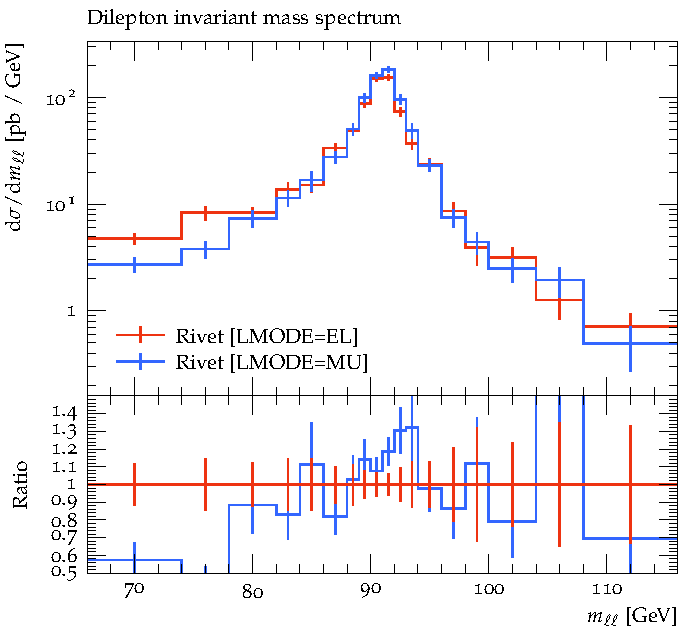
\includegraphics[width=0.49\textwidth]{figures/mass_ll.pdf}
\end{center}

You should find a $Z$-boson resonance similar to the plot above. 
In case you are missing the axis labels, try the
\begin{verbatim}
  export RIVET_ANALYSIS_PATH=$PWD
\end{verbatim}
trick to let Rivet know about where to look for the \verb|plot| file with the 
cosmetic settings that we have prepared for you. 
Alternatively, you can pass this file directly to the
plotting command using the \verb|-c| flag.
Does the ratio between the two predictions match your expectation?



\section{Bare level vs dressed level}

It turns out leptons lose energy through photon radiation and the effect is much more pronounced
for electrons due to their lower invariant mass. What we have plotted is the invariant mass of
the dilepton spectrum constructed from leptons at the so-called \emph{bare level}, i.e.\
after photon radiation, which explains why the electron-pair lineshape deviates from the muon-pair version.
Luckily, Rivet offers more complex projections that implement experimental strategies, e.g.\ for
lepton dressing, heavy-flavour tagging or mass-windowing and so on.
For instance, the \verb|DressedLeptons| projection dresses the bare lepton four-momentum 
with all photon four-momenta, within a given cone size (typically 0.1) in order to recover 
energy losses from QED final-state radiation (FSR). Leptons whose four-momenta have been
corrected in this way are referred to as being reconstructed at the \emph{dressed level}.
The \verb|DressedLeptons| constructor 
takes the following arguments:
\begin{small}
\begin{verbatim}
  DressedLeptons leps(photon FS, bare-lepton FS, dressing-cone size, optional selection cuts);
\end{verbatim}
\end{small}
This is the recommended procedure to define leptons at the particle level, 
since it is more robust against generator differences in the modelling of QED FSR.
Let's see this in action!

\begin{exercise}
Implement an \emph{additional} plot of the dressed-level dilepton invariant mass
spectrum in the \verb|cc| file, with otherwise equivalent kinematic requirements
on the leptons. Re-compile, re-run and re-plot to check the effect.
\end{exercise}

At the end of the exercise you should be able to produce two plots similar to
the ones on the next page. The one on the left-hand side shows the dilepton
invariant mass spectrum constructed from leptons at the bare level, while 
the one on the right-hand side shows the same spectrum constructed from
leptons at the dressed level. The compensating effect of the dressing
procedure should be clearly visible when comparing the two ratios.

\clearpage

\begin{center}
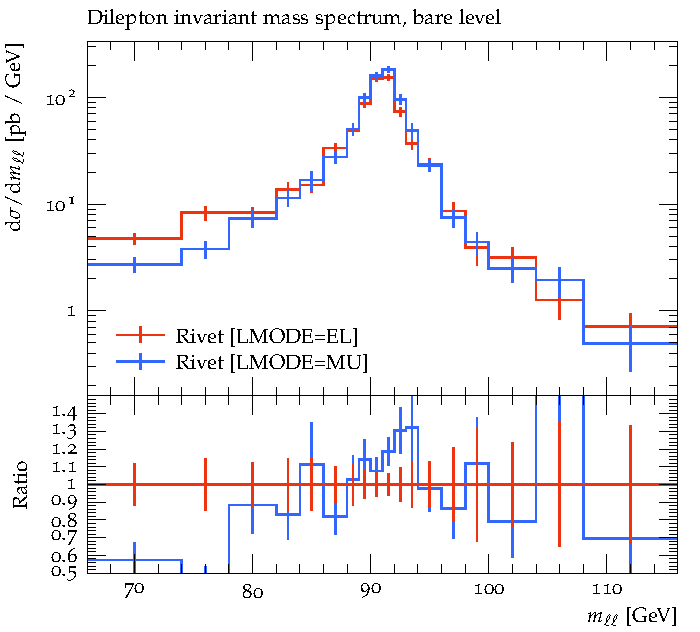
\includegraphics[width=0.49\textwidth]{figures/mass_ll_bare.pdf}
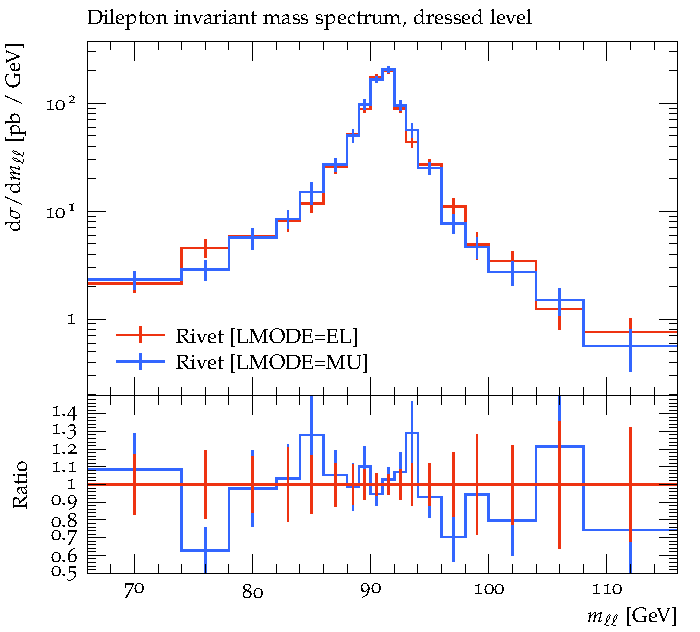
\includegraphics[width=0.49\textwidth]{figures/mass_ll_dressed.pdf}
\end{center}


\section{Jet-based observables}

Rivet has a lot of neat and flexible built-in support to make your life easier
and in this section we will look into how to make use of the most common features.
We will start by constructing our own jet collection.
Some general advice upfront: avoid coding up built-in methods from scratch
as this can be highly error prone! Besides, why reinvent the wheel?


Jets are typically constructed with the \texttt{FastJet} program.
Rivet has a \verb|FastJets| projection which uses the \texttt{FastJet} 
program internally. The constructor could look like this:
\begin{small}
\begin{verbatim}
  FastJets jets(input FS, FastJets::KT, 1.0, JetAlg::Muons::NONE, JetAlg::Invisibles::NONE);
\end{verbatim}
\end{small}
The first argument is the \verb|FinalState|-based input collection of particles to be clustered.
The second and third argument specify the clustering algorithm and associated jet-radius parameter.
The last two arguments are optional and can be used to reflect experimental strategies for
how to deal with muons or invisibles particles in the clustering.
Possible values are \verb|NONE|, \verb|DECAY|, \verb|ALL|; the default being 
to include all muons (\verb|Muons::ALL|) but to exclude all invisible particles (\verb|Invisibles::NONE|).
Similar to the \verb|particlesByPt()| method we encountered earlier, the \verb|FastJet| projection
comes with an equivalent \verb|jetsByPt()| method. It takes an optional \verb|Cuts| argument as well, 
which allows to efficiently select a subset of the jets that pass certain fiducial requirements.
Rivet supports auto-conversion to and from \verb|fastjet::pseudoJet| as well as its own \verb|Jet| class,
i.e.\ it also does not matter which version is passed into the various built-in functions that Rivet has to offer.
As always, remember to add the relevant include statement
\begin{verbatim}
  #include "Rivet/Projections/FastJets.hh"
\end{verbatim}
near the top of the routine if it is not already included.


\begin{exercise}
Select events with $66\,\text{GeV} < m_{\ell\ell} < 116\,\text{GeV}$ at using letpons
defined at the dressed level.
Using the anti-$k_\text{T}$ algorithm with a jet-radius parameter of 0.4,
cluster all final-state particles within $|\eta| < 4.9$, 
except for muons and invisible particles.
Select all jets with $p_\text{T} > 10$\,GeV and within $|y| < 4.5$,
then count them to plot the exclusive jet multiplicity.
Additionally, add a plot of the scalar jet $p_\text{T}$ sum.
The latter is often referred to as $H_\text{T}$ and is a measure
for the amount of hadronic activity in the event.
Run this setup separately for each lepton channel and compare the curves.
\emph{Optional:} You may find Rivet's built-in \verb|sum| function
helpful which takes three arguments:
\begin{verbatim}
  sum(iterable container, property, initial value)
\end{verbatim}
and returns a scalar or vector depending on the property called
on the elements in the container.
\end{exercise}

At the end of this exercise, you be able to produce two plots that
look something like this:

\begin{center}
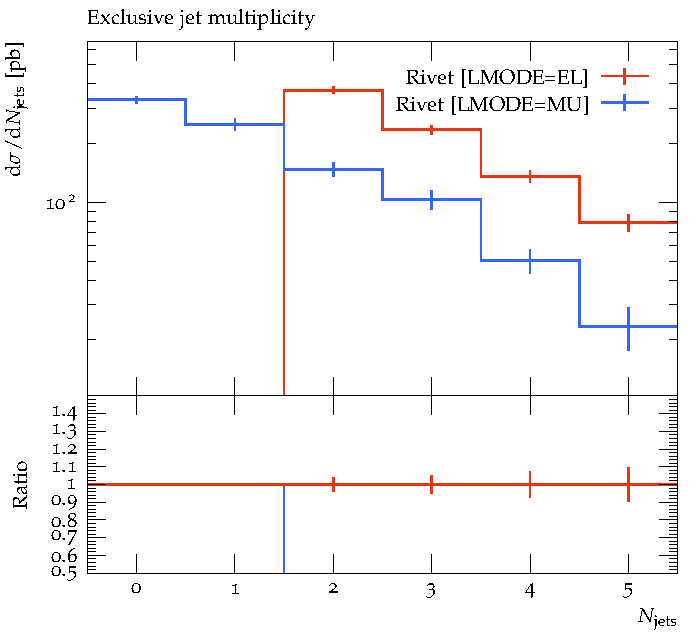
\includegraphics[width=0.49\textwidth]{figures/jets_excl_no_olr.pdf}
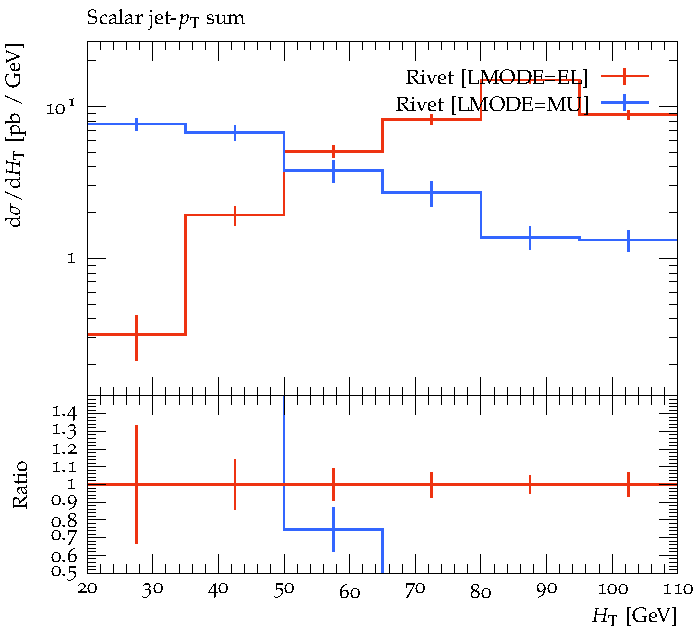
\includegraphics[width=0.49\textwidth]{figures/HT_no_olr.pdf}
\end{center}

The differences between the electron and the muon channel are rather striking,
but expected considering what goes into the jet clustering. 
Out of all the visible particles within the pseudorapidity acceptence,
only the muons have been removed while the electrons are included
into the jet-clustering algorithm as though they were jets.
In some sense this is very similar to how electrons and hadrons would leave 
an energy deposit inside a calorimeter, while muons tend to pass through it
and would need to be detected via a dedicated tracker.

At the particle level one has full flexibility about what to include in the clustering
and what not. From the point of view of e.g.\ ATLAS and CMS, however,
usually everything is a jet to start with: 
Most visible particles produced in an event eventually hit the calorimeter and
detector-level jets can be constructed from the energy depositions in the calorimeter cells.
Additional dedicated sub-detectors may exist to identify e.g.\ electron, photon or muon candidates
and as a result, a given physics object can appear in several of the object collections
reconstructed using the various detector components.
This is why ``overlap removal'' is a thing in experimental analyses.
In its simplest form, the objects from the dedicated sub-detectors are preferred, 
e.g.\ due to superior resolution or selection efficiency, and so the candidates
from other object collections (reconstructed with less precise detector components)
which fall into the same fiducial phase space are simply removed from the final state
in those object collections.

\begin{exercise}
Modify the \verb|cc| file to remove all jets that are within $\Delta R < 0.4$
of a selected dressed-level electron or a dressed-level muon, 
then re-compile, re-run, re-plot and re-compare.
\emph{Optional:} You may find Rivet's built-in \verb|discardIfAnyDeltaRLess| function
helpful which takes three arguments:
\begin{verbatim}
  discardIfAnyDeltaRLess(input container, reference container, cone size)
\end{verbatim}
which returns a copy of the input container with all elements removed
that fall within a cone of the specified size with any of the elements
of the reference container. An \verb|i| added in front of the function
name will modify the input container in place without making a new copy.
\end{exercise}

At the end of this exercise you should be able to obtain plots similar 
to those shown on the next page, where the kinematic distributions 
are now compatible between the electron and the muon channel.
Of course you are free to code up the overlap-removal prescription
using a standard C++ for loop, but notice how much easier to read
the code becomes when pushing the boring bits of experimental
strategy into Rivet's built-in functions to leave more headspace
for physics. 
There is another common experimental strategy that emphasises 
this point even better, which we will focus on in the next section.

\begin{center}
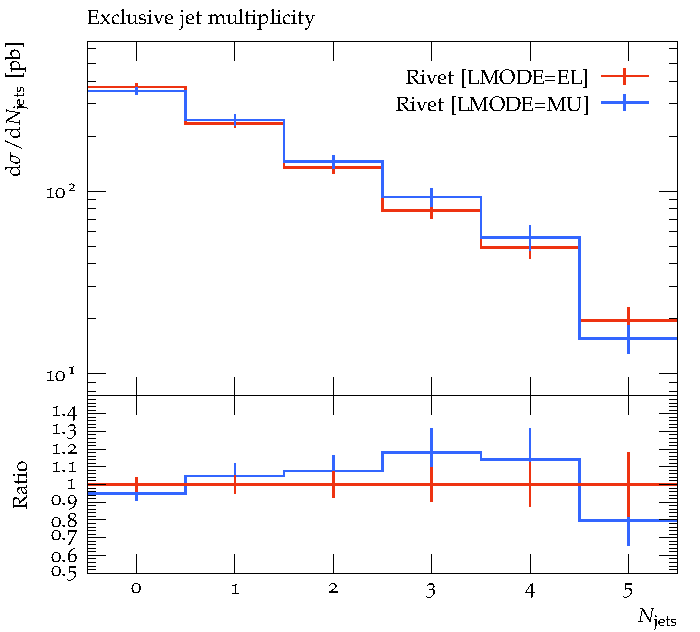
\includegraphics[width=0.49\textwidth]{figures/jets_excl.pdf}
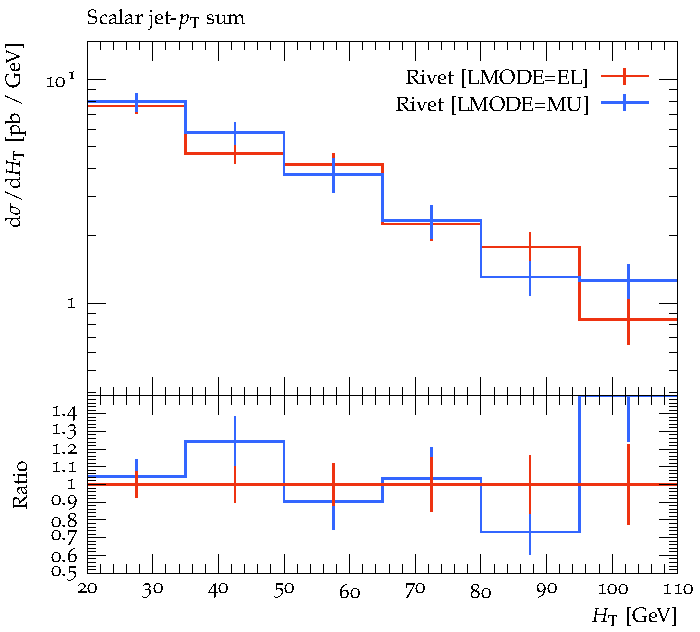
\includegraphics[width=0.49\textwidth]{figures/HT.pdf}
\end{center}

\section{Heavy-flavour tagging}

The preferred way to define $b$-jets or $c$-jets at the particle level 
is to ghost-associate heavy-flavour hadrons to the jets.
The idea behind this strategy is to ``let the clustering algorithm decide''
this in an infrared-safe way.
Heavy-flavour hadrons are not stable and hence not included in the jet clustering,
which is based on stable final-state particles.
``Ghost association'' is a technique whereby these hadrons are manually added to the collection of
input particles that are to be clustered, but with their 4-momenta scaled down to (effectively) meaningless size,
such that the anti-$k_\text{T}$ algorithm can just pull them into a jet as it sees fit.

No need to stress: Rivet automatically implements this for you behind the scenes!
`Is my jet a $b$-jet?' becomes as simple as
\begin{verbatim}
if (myJet.bTagged()) ...
\end{verbatim}
One can even use the familiar \verb|Cuts| argument to refine the tagging further:
\begin{verbatim}
if (myJet.bTagged(Cuts::abseta < 2.5)) ...
\end{verbatim}
Access to the tagged hadrons is also provided via \verb|myJet.bTags()| and
needless to say that similar functions for $c$-tagging are available as well.
Let's practice this!

\begin{exercise}
Modify the \verb|cc| file to add a plot of the exclusive $b$-jet multiplicity.
\emph{Optional:} You may find Rivet's built-in \verb|count| function
helpful which takes up to two arguments
\begin{verbatim}
  count(input container, selection criterion)
\end{verbatim}
where the selection criterion could be a \verb|Cuts| argument or a C++ function
that is to be called on the elements in the input container, such as
Rivet's built-in \verb|hasBTag(Cuts)| method.
\end{exercise}

At the end of this exercise, you should have produced a plot similar to
the one shown on the next page. Notice how much more readible the code
becomes when relying on the built-in functions. A typical implementation
of ghost-association can easily take somewhere between 200-300 lines of C++
and so re-inventing the wheel here would not only clutter the routine 
but also boost the chances for bugs to be introduced.

\begin{center}
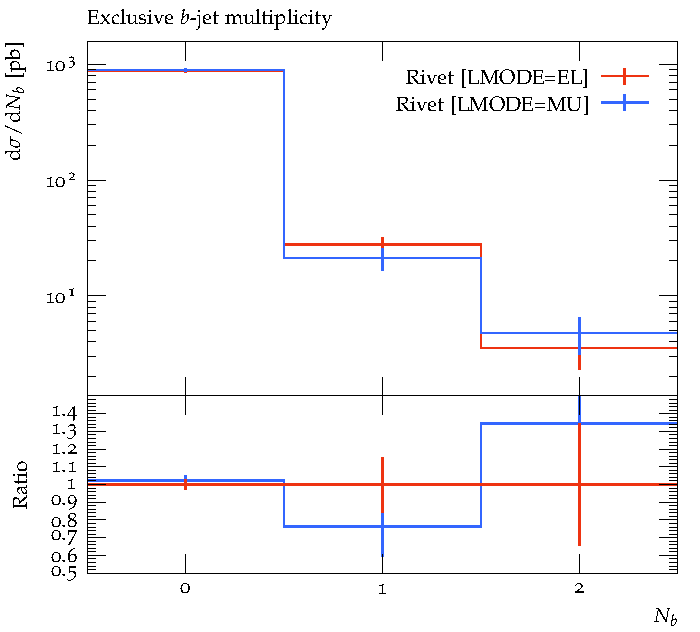
\includegraphics[width=0.49\textwidth]{figures/bjets_excl.pdf}
\end{center}

\section{Scale uncertainties using on-the-fly variation weights}

The events provided for you in the HepMC file were produced using on-the-fly variations
of the factorisation and renormalisation scale in matrix element and parton shower.
In fact, the setup also includes these variations for the case where only the matrix element
scales were varied but not the scales in the parton shower.
In this exercise we want to use the variation weights to estimate the 
corresponding scale uncertainties and add some uncertainty bands to our plot.

Fortunately, we already have all the ingredients to do this, since Rivet will
automatically book one histogram per weight variation for you behind the scenes.
Out-of-the-box multiweight support is one of the main new features of the Rivet 3 release series!
In order to make better use of the available statistics, we recommend to re-run the routine
\emph{without} an \verb|LMODE| option, so as to accept either lepton-flavour channel 
in the same run. Consider running one of the routines included natively in the Rivet 
release to be able to compare against data as well, such as \verb|ATLAS_2017_I1514251|,
the 13\,TeV $Z$+jets measurement~(\href{https://arxiv.org/abs/1702.05725}{arXiv:1702.05725}) 
from the ATLAS experiment for instance.

Try plotting this without passing the \verb|--no-weights| flag to the \verb|rivet-mkhtml| command.
What you should see is something like the following:

\begin{center}
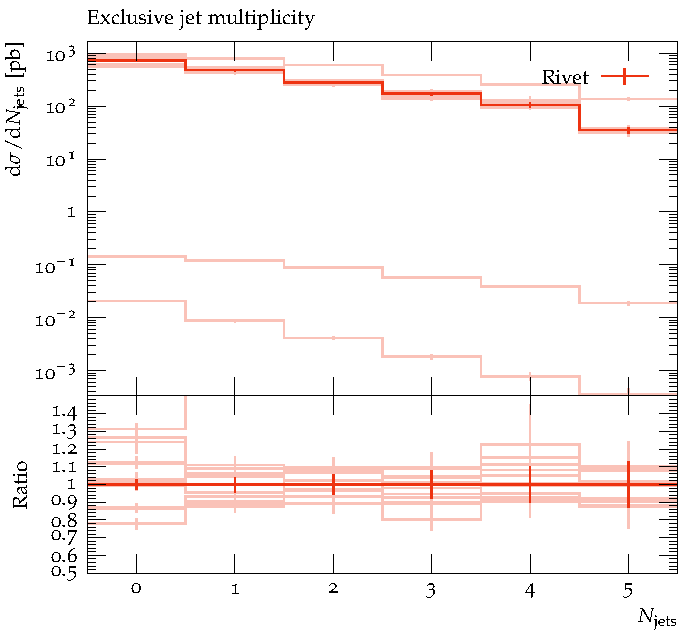
\includegraphics[width=0.49\textwidth]{figures/jets_excl_all_weights.pdf}
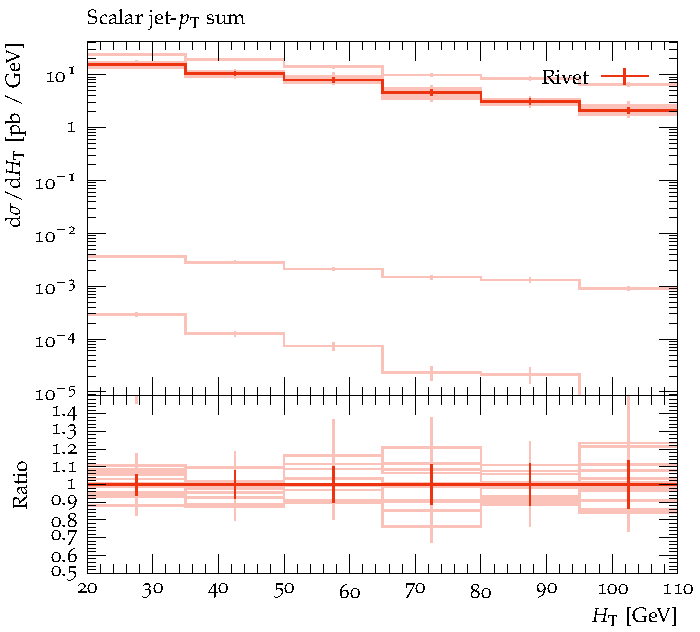
\includegraphics[width=0.49\textwidth]{figures/HT_all_weights.pdf}
\end{center}

The default behaviour is to superimpose the available variation weights in a lighter
shading along with the central value. This already gives an idea of the spread of
the variations, but it also highlights that there seem to be some variation weights 
in the setup that correspond to some auxiliary quantity which isn't mean to be used
for histogramming. These are the two curves which lie at least a factor $\mathcal{O}(10^4)$
below the central value. There is currently no agreed upon standard for how to label
weights and so the Rivet default behaviour is to be as inclusive as feasible when
it comes to weight variations. However, it also provides some functionality to filter
out a specific subset of the weights. In the following we will look at a few examples
for how to deal with weights when using the plotting scripts, but in principle similar
options are also available to (de-)select weights already at run time 
(cf. \verb|rivet --help| for the available flags).

Let's take a look at what sort of variation weights are included in the setup:
\begin{verbatim}
  import rivet, yoda
  print set([ rivet.extractWeightName(name) for name in yoda.read("Rivet.yoda") ])
\end{verbatim}
Here we are using the Python API of YODA to load the output file, loop over all
the objects in the file and to use Rivet's Python API to extract the weight names.
The result is then turned into a Python \verb|set| in order to remove duplicate entries in the array.
%The result should look something like:
%\begin{verbatim}
%  {'', 'ME_ONLY_MUR1_MUF1_PDF261000', 'MUR1_MUF0.5_PDF261000_PSMUR1_PSMUF0.5', 'NTrials', 'ME_ONLY_MUR0.5_MUF0.5_PDF261000_PSMUR0.5_PSMUF0.5', 'ME_ONLY_MUR2_MUF1_PDF261000_PSMUR2_PSMUF1', 'MUR0.5_MUF0.5_PDF261000_PSMUR0.5_PSMUF0.5', 'MUR1_MUF1_PDF261000', 'MUR2_MUF2_PDF261000_PSMUR2_PSMUF2', 'MUR1_MUF2_PDF261000_PSMUR1_PSMUF2', 'ME_ONLY_MUR1_MUF2_PDF261000_PSMUR1_PSMUF2', 'WeightNormalisation', 'ME_ONLY_MUR0.5_MUF1_PDF261000_PSMUR0.5_PSMUF1', 'MUR2_MUF1_PDF261000_PSMUR2_PSMUF1', 'ME_ONLY_MUR1_MUF0.5_PDF261000_PSMUR1_PSMUF0.5', 'MEWeight', 'MUR0.5_MUF1_PDF261000_PSMUR0.5_PSMUF1', 'ME_ONLY_MUR2_MUF2_PDF261000_PSMUR2_PSMUF2'}
%\end{verbatim}
You will notice that most of the scale variations
seem to follow the pattern \verb|MUR*_MUF*_PDF261000| at their core where the wild card is either \verb|0.5|,
\verb|1| or \verb|2|. We can use this observation to select all the variation weights
that pass the corresponding regular expression
\begin{verbatim}
  rivet-mkhtml --errs Rivet.yoda:"Variations=MUR.*_MUF.*_PDF261000"
\end{verbatim}
This will essentially produce the same plots as above but without the outliers
at the bottom of the canvas. Let's take it one step further and attempt to combine
the weights into a band. In general, the prescription for how to combine the
scale and PDF variations depends on the specific setup, 
in particular the PDF set used and the precise format of the weight names.
The combination strategy needs to be defined by the user in the end, but Rivet
supports some very basic prescriptions out of the box. 
The simplest thing one could ask is to combine the weights into en uncertainty band
based on the envelope of the variations. For instance, we could ask Rivet to work out
the envelope for the same regular expression like so
\begin{footnotesize}
\begin{verbatim}
  rivet-mkhtml --errs Rivet.yoda:"Variations=MUR.*_MUF.*_PDF261000 BandComponentEnv=MUR.*_MUF.*_PDF261000"
\end{verbatim}
\end{footnotesize}
which will produce something like the following:

\begin{center}
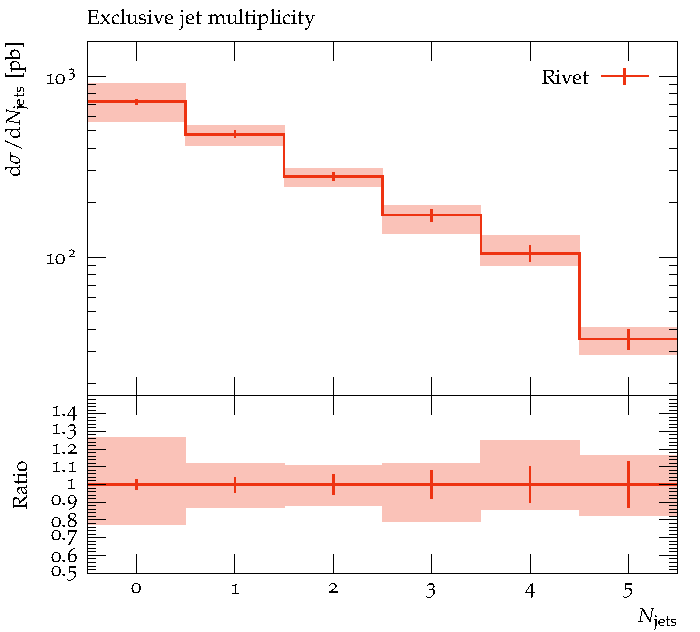
\includegraphics[width=0.49\textwidth]{figures/jets_excl_all_band.pdf}
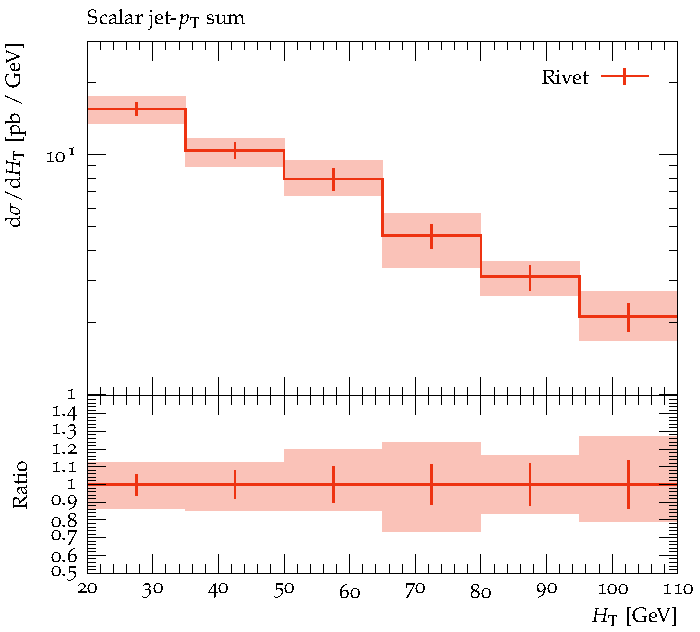
\includegraphics[width=0.49\textwidth]{figures/HT_all_band.pdf}
\end{center}

This is not too bad for a first quick look at the rough size of the uncertainties,
but we can do better with a little bit more work. 
In particular, if we take another close look at the list of weight names available
for this setup, we see versions with and without an additional \verb|ME_ONLY_| prepended
to the name. The difference between these is that the scales were only varied in
the matrix element or coherently in both matrix element and parton shower.
It might be interesting to separate these out into two bands.
While this can in principle also be done on the command line, let us play around
with the Python API a bit more and use it implement a simple weight-combination
prescription ourselves. The goal of the next exercise is to split the output file
into separate copies that differ in the size of their combined uncertainty,
as indicated by the name suffix \verb|stat_only|, \verb|stat_MEonly| 
or \verb|full_band| respectively.


\begin{exercise}
Complete the code in the \verb|makeBands.py| skeleton.
\end{exercise}

Once the weights are combined into bands, it is straightforward
to superimpose different bands using the usual plotting
scripts. For clarity, it is useful to play around with different
colours, band styles or opacity levels. One possible solution
is the following:
\begin{verbatim}
  DBLUE="blue!90!white"
  MBLUE="blue!60!white"
  LBLUE="blue!30!white"
  COMMON_TAGS="RatioPlotSameStyle=1:ErrorBars=0:ErrorBands=1:ErrorBandOpacity=0.5"
  MEPS_STYLE=$COMMON_TAGS:ErrorBandColor=$LBLUE:LineColor=$LBLUE
  ME_STYLE=$COMMON_TAGS:ErrorBandColor=$MBLUE:LineColor=$MBLUE
  STAT_STYLE=$COMMON_TAGS:ErrorBandStyle=hlines:ErrorBandColor=$DBLUE:LineColor=$DBLUE

  rivet-mkhtml --errs -o plots_with_bands \
  Rivet_full_band.yoda:$MEPS_STYLE:"Title=ME+PS scales \$\\oplus\$ stats" \
  Rivet_stat_MEonly.yoda:$ME_STYLE:"Title=ME scales \$\\oplus\$ stats" \
  Rivet_stat_only.yoda:$STAT_STYLE:"Title=stats only"
\end{verbatim}
which you can run on the command line or copy into a bash script first.
The above implementation also gives an idea for how to do a few more
fancy style customisations with the plotting scripts. 
The result should look something like this

\begin{center}
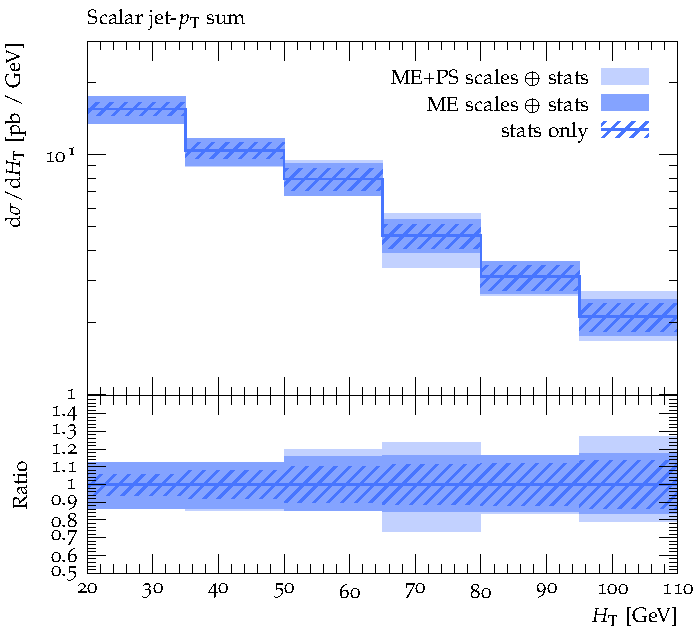
\includegraphics[width=0.49\textwidth]{figures/HT_bands.pdf}
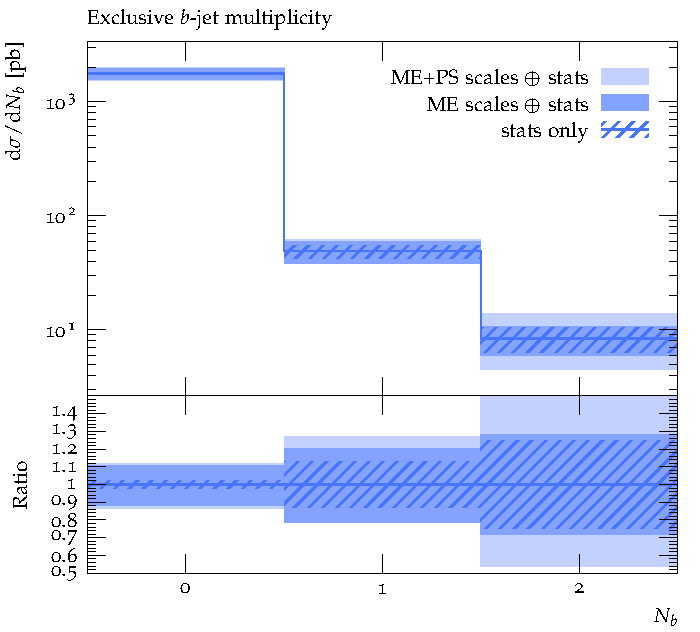
\includegraphics[width=0.49\textwidth]{figures/bjets_excl_bands.pdf}
\end{center}

Even with this small event sample, it can be seen that the parton-shower-based
scale variations become relevant in the more exclusive regions of phase space.

At this stage you should be familiar with the basics of running Rivet,
be able to write a custom routine, make some first plots 
and even construct uncertainty bands from the weight variations.
If you have some spare time, feel free to have a go at the next exercise
which plays a bit more with invisible particles and fiducial definitions.


\section{Optional: A balancing act in the transverse plane}

In the general-purpose detectors at the LHC, a momentum imbalance 
in the transverse plane can be used to infer the presence
of particles have otherwise escaped direct detection in the detector.
When designing a fiducial measurement phase space, it is important 
to bear in mind that the imbalance could be due to SM neutrinos or BSM invisibles,
and that it is much preferable to avoid model-dependent assumptions 
about the composition of missing $p_\text{T}$ in a measurement.
The particle-level definition of missing $p_\text{T}$ should ideally match what is being done
at the detector level, where the imbalance would typically be estimated
by taking the negative of the vector sum over all visible particles in an event.
Rivet's \verb|MissingMomentum| projection calculates missing $p_\text{T}$ (or $E_\text{T}$) for you in this way. 
If a detector does not cover the full phase space, 
remember that a fiducial \verb|FinalState| can also be passed as an argument.

\begin{exercise}
Imagine an experimental setup for which neutrinos are invisible, 
muons can be detected within $|\eta| < 2.5$, 
while the jets produced in association with the
boson can be detected within $|\eta| < 4.9$.
Construct the missing $p_\text{T}$ using Rivet's \verb|MissingMomentum| projection
(\emph{i}) from all visible particles in the event
(\emph{ii}) from all visible particles that can be detected by this setup.
Consider introducing a new option \verb|INVMODE=STRICT,FIDUCIAL| to steer the analysis logic, 
depending on whether the imbalance should come (\emph{i}) strictly from invisibles or
(\emph{ii}) anything the detector cannot `see'.

\emph{Hint:} The following might come in handy: 
\begin{verbatim}
apply<MissingMomentum>(event, "pTmiss").missingPt()
\end{verbatim}
\end{exercise}

Implementing the logic for this is greatly simplified when relying on
the \verb|MissingMomentum| projection, but since it amounts to
making the routine also work with $W$+jets events, 
it might still require a bit of thinking. 
Assuming the routine is run with both \verb|INVMODE| options
in the same run, this can be plotted in following way
\begin{verbatim}
  SUB1="ReplaceOption[INVMODE=STRICT]=invisibles only"
  SUB2="ReplaceOption[INVMODE=FIDUCIAL]=invisibles and out-of-acceptance muons"
  rivet-mkhtml --no-weights --errs wjets.yoda:"" PLOT:"$SUB1":"$SUB2"
\end{verbatim}
where the two \verb|ReplaceOption[option=value]=replacement string| tags could 
either be added directly to the \verb|plot| file or be passed on the command line like above. 
This is just a small cosmetical tweak to make the legend a bit more readable.
The result should look somewhat like this:

\begin{center}
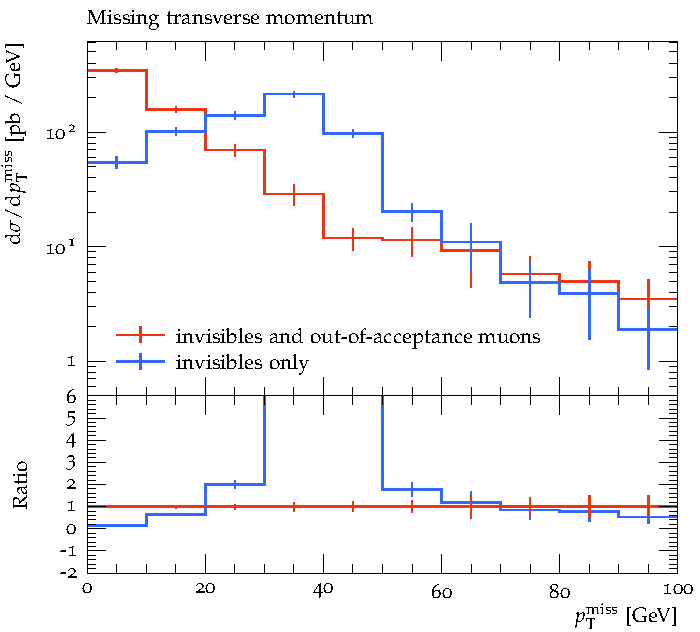
\includegraphics[width=0.49\textwidth]{figures/pTmiss.pdf}
\end{center}

What does the difference between the two curves imply
for a measurement of missing transverse momentum?

\section{Summary}

In this tutorial, we covered various practical aspects of a typical truth-level analysis
as well as common issues to do with fiducial particle-level definitions.
A Rivet routine is a snippet of C++ code that exactly implements the analysis logic.
We wrote a simple routine to analyse events of weak-boson production in association
with jets using Rivet. 
(An example solution can be found in the repository when listing also the hidden files.)
Along with making the measurement results publicly available on HEPData,
providing a Rivet routine is an important aspect of analysis preservation
that helps to maximise the impact of the analysis results as well as
making them overall more useful to the community.

\end{document}

